\documentclass[dvipdfmx,a4paper,12pt]{jsarticle}

\title{Learning a Boolean function}
\author{伊藤 碧己}

\usepackage[dvipdfmx]{graphicx}
\usepackage{amsmath}
\begin{document}
\maketitle

%メモ:
%・termとclauseの使い分け→DNFでは項(term),CNFでは節(clause)と表現されている
%・DNFをSAT問題として簡単に表現できる理由

\begin{figure}[htbp]
  \centering
  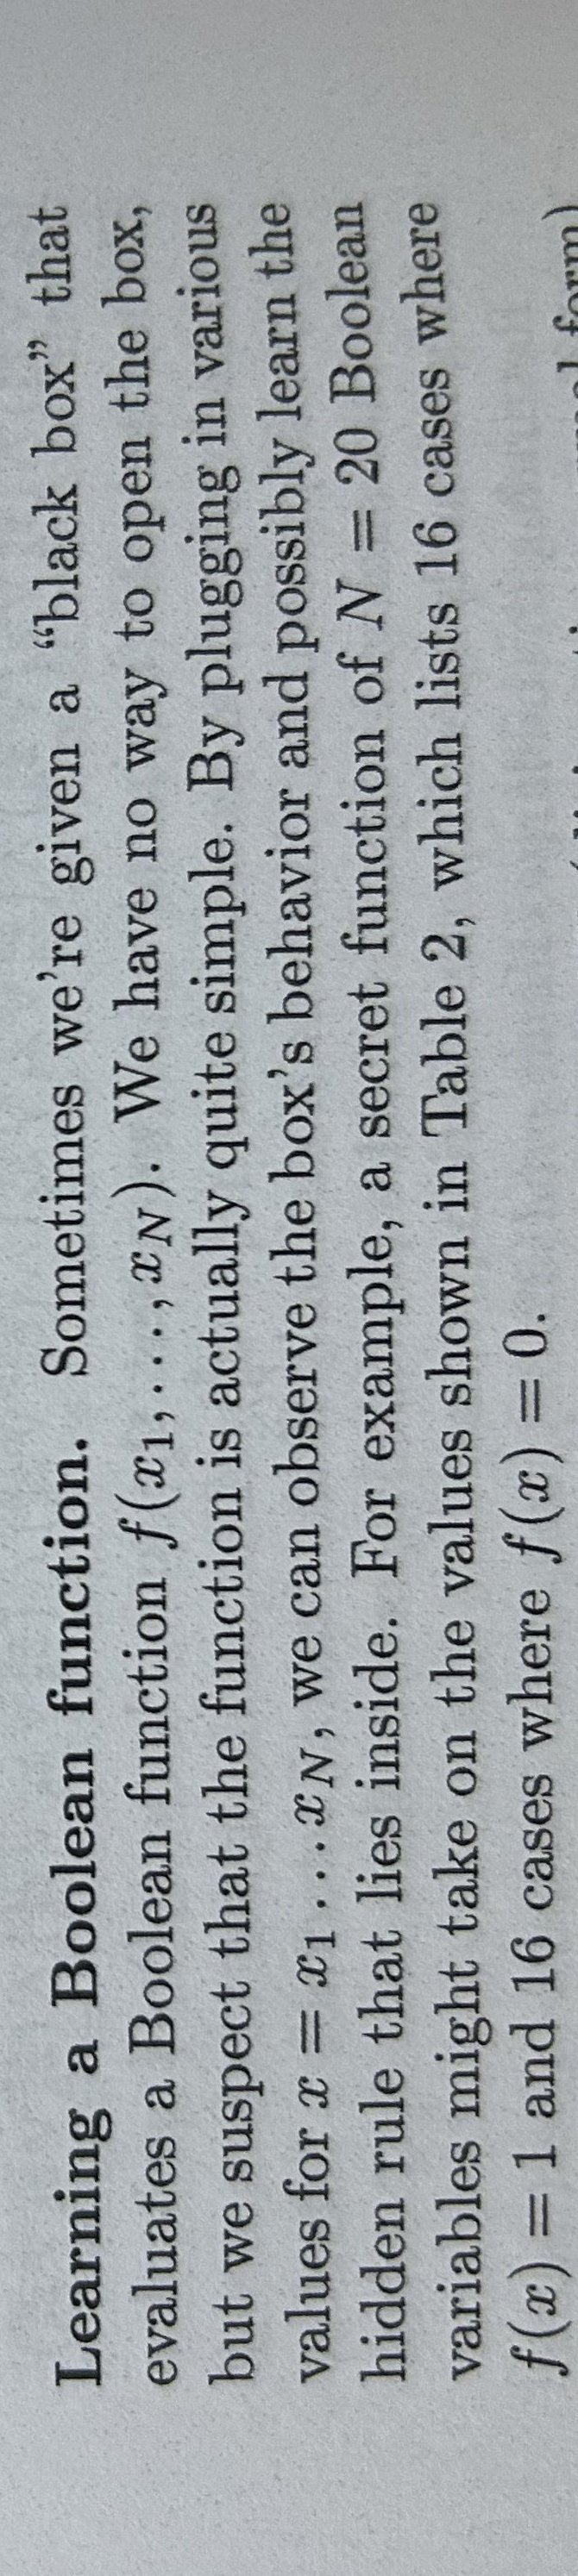
\includegraphics[width=28mm,angle=270]{images/1.jpg}
\end{figure}
\textbf{ブール関数の学習.}
私たちは時々"ブラックボックス "を与えられる,ブール関数$f(x_{1},...,x_{N})$を評価する.私たちはその箱を開ける方法を持たない,しかし私たちは考える,その関数は実際には非常に単純なものであると.$x = x_{1}...x_{N}$に様々な値を代入することで,私たちはその箱の振る舞いを観察することができ,その中にある隠れたルールを学ぶことができるかもしれない.例えば、$N = 20$のブール変数の秘密の関数は表2に示すような値をとるかもしれない,$f(x) = 1$である16のケースと$f(x) = 0$である16のケースが列挙されている.
\begin{figure}[htbp]
  \centering
  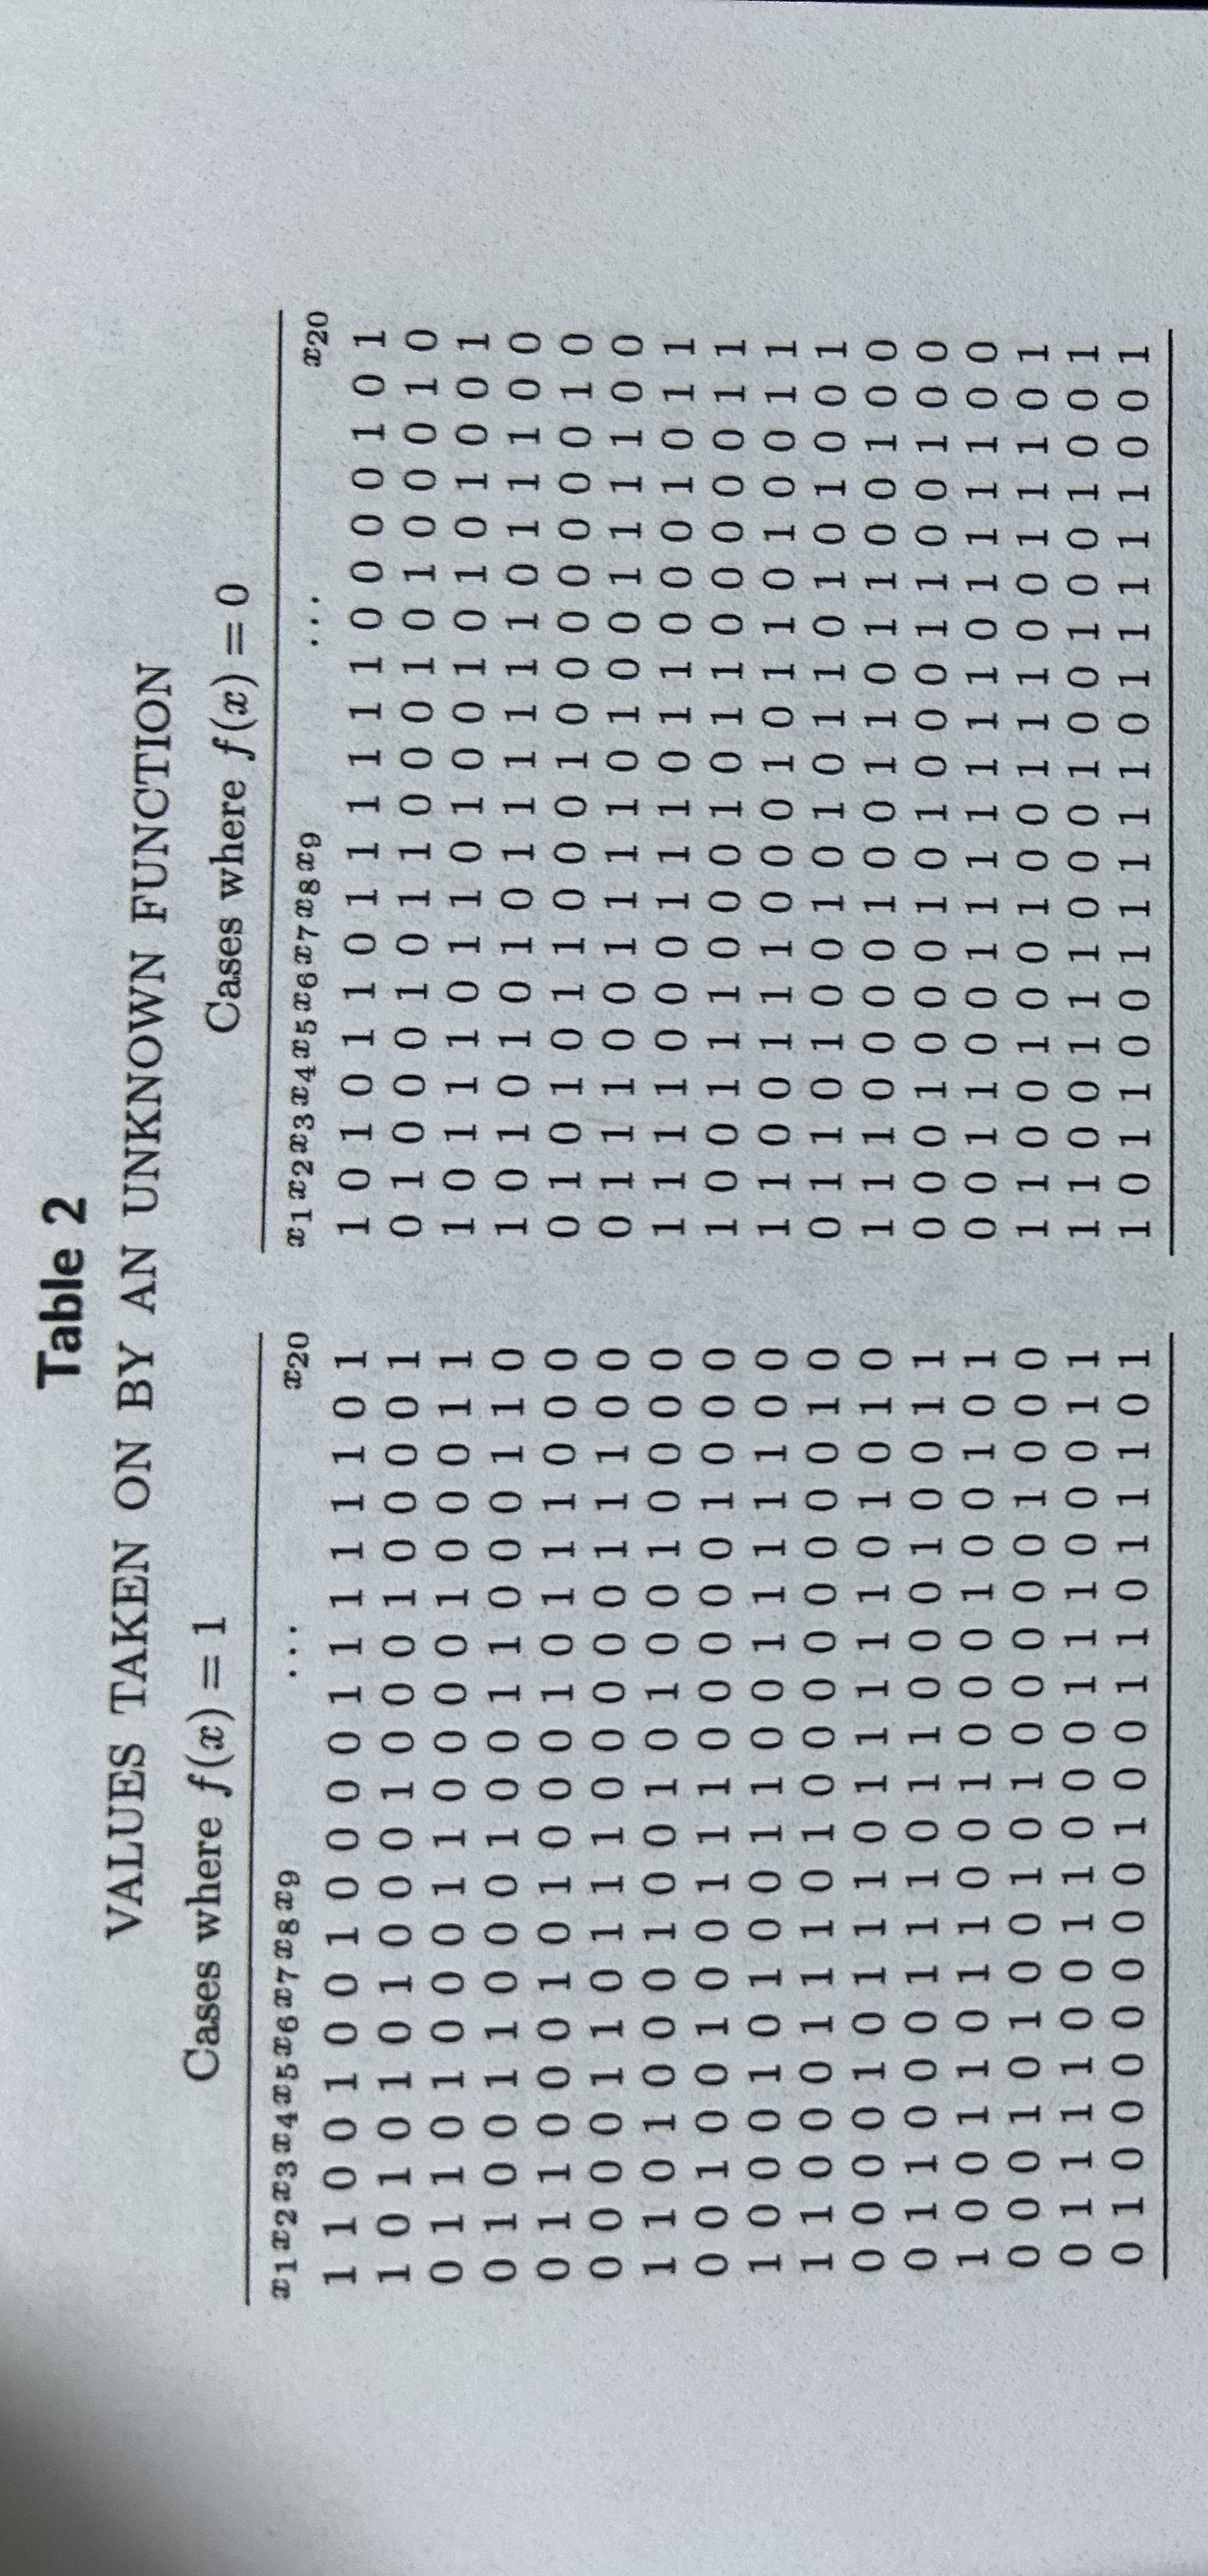
\includegraphics[width=55mm,angle=270]{images/table2.jpg}
\end{figure}

%%%%%%%%%%%%%%%%%%%%%%%%%
\newpage
\begin{figure}[htbp]
  \centering
  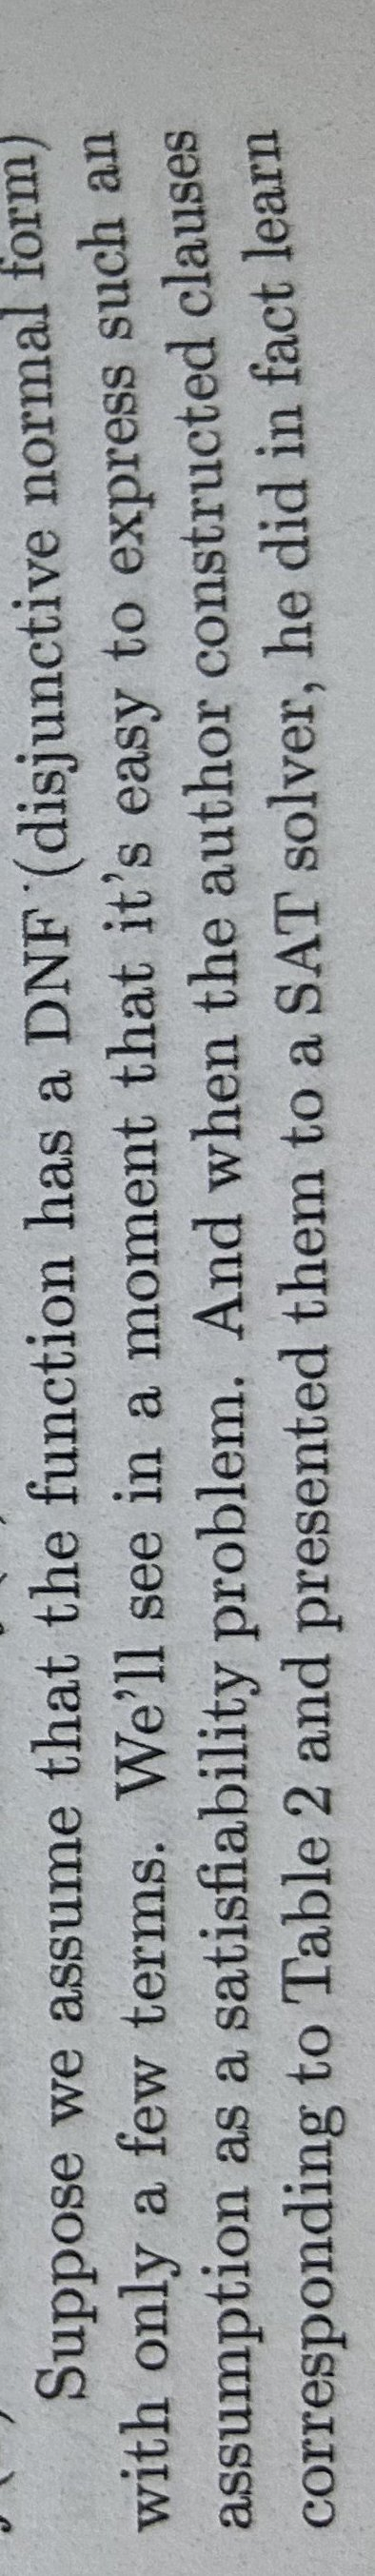
\includegraphics[width=20mm,angle=270]{images/2.jpg}
\end{figure}
\begin{figure}[htbp]
  \centering
  
\includegraphics[width=12.5mm,angle=270]{images/3.jpg}
\end{figure}
私たちはその関数がDNF(選言標準形)であると仮定するとしよう,いくつかの項のみを持つ.私たちはすぐに分かる,このような仮定を充足可能性問題として表現するのは簡単であると.
そして,筆者が表2に対応する節を構築し,SATソルバーに提示したところ,彼は実際に,ほとんど即座に知った,非常に単純な式がすべてのデータと一致すると:
\setcounter{equation}{26}
\begin{equation}
f(x_{1},...,x_{20}) = \bar{x}_{2}\bar{x}_{3}\bar{x}_{10}\lor\bar{x}_{6}\bar{x}_{10}\bar{x}_{12}\lor x_{8}\bar{x}_{13}\bar{x}_{15}\lor \bar{x}_{8}x_{10}\bar{x}_{12} 
\end{equation}  
%\footnote{最も簡単にDNFを作成するには,表2の各行に対し,1なら正リテラル,0なら負リテラル}
\begin{figure}[htbp]
  \centering
  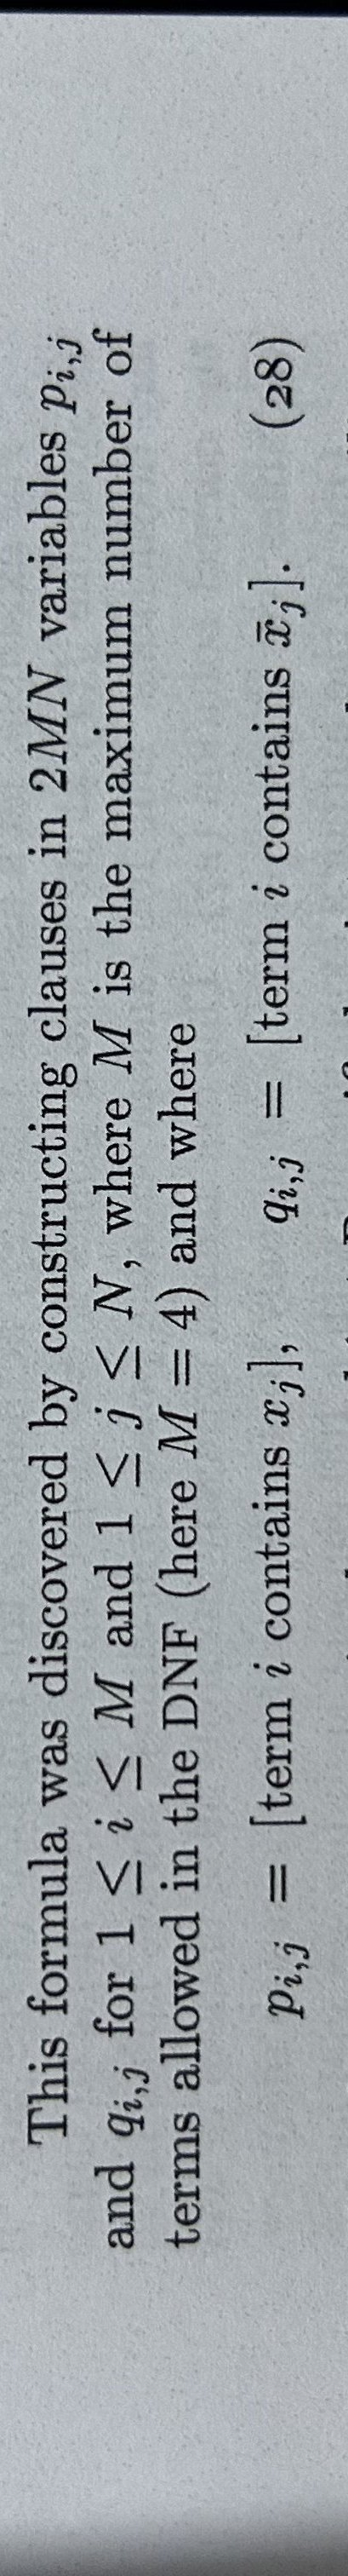
\includegraphics[width=18.5mm,angle=270]{images/2-2.jpg}
\end{figure}

この式は,$2MN$の変数$p_{i,j}$と$q_{i,j}$で節を構成することによって発見された,
ここで$1 \le i \le M$ かつ $1 \le j \le N$である,
$M$はDNFで許される項の最大個数(ここでは$M = 4$)である,また
\begin{equation}
p_{i,j} = [ 項iはx_{j}を含む],q_{i,j} = [ 項iは\bar{x}_{j}を含む] 
\end{equation}
%%%%%%%%%%%%%%%%%%%%%%%%%
\clearpage
\begin{figure}[htbp]
  \centering
  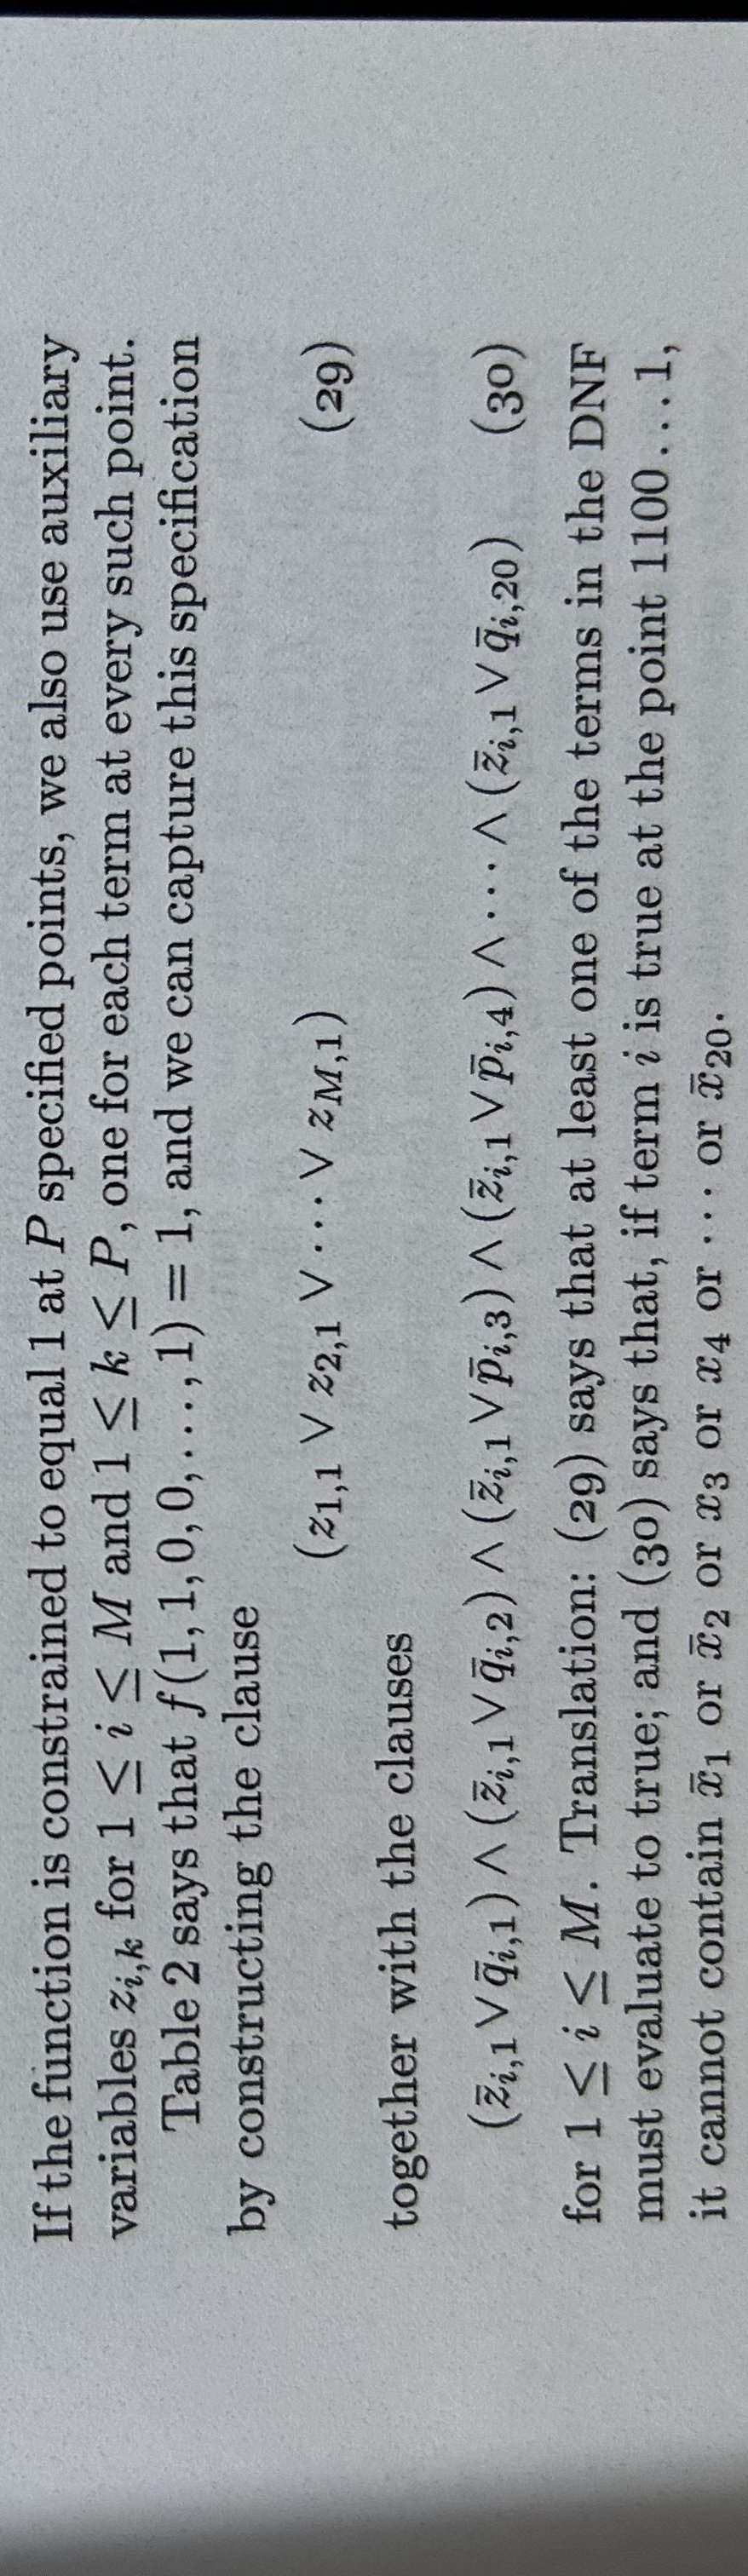
\includegraphics[width=38mm,angle=270]{images/2-3.jpg}
\end{figure}
もし関数が$P$個の特定の点で1に等しくなるように制約されているなら,\footnote{f(x1,x2,...xn)=1となるブール変数の組み合わせがP個ある,という意味}加えて補助変数$z_{i,k}$を用いる,$1 \le i \le M$かつ$1 \le k \le P$,そのような全ての点について各項に1つずつ.

 表2は,$f(1,1,0,0,...,1)=1$であると述べており,私たちはこの指定を捕らえることができる,次の節を構成することによって
 \begin{equation}
(z_{1,1} \lor z_{2,1} \lor ・・・ \lor z_{M,1})
\end{equation}  
次の節たちとともに
  \begin{equation}
(\bar{z}_{i,1} \lor \bar{q}_{i,1}) \land (\bar{z}_{i,1} \lor \bar{q}_{i,2}) \land (\bar{z}_{i,1} \lor \bar{p}_{i,3}) \land (\bar{z}_{i,1} \lor \bar{p}_{i,4}) \land ・・・ \land (\bar{z}_{i,1} \lor \bar{q}_{i,20})
\end{equation}  
$1 \le i \le M$に対して.
注釈:(29)は示す,DNFの項のうち少なくとも1つは真と評価されなければならない;そして
(30)は示す,もし項$i$が点1100...1で真ならば,それは$\bar{x}_{1}$または$\bar{x}_{2}$または$x_{3}$または$x_{4}または...$または$\bar{x}_{20}$を含むことはできない.

%%%%%%%%%%%%%%%%%%%%%%%%%
\clearpage
\begin{figure}[htbp]
  \centering
  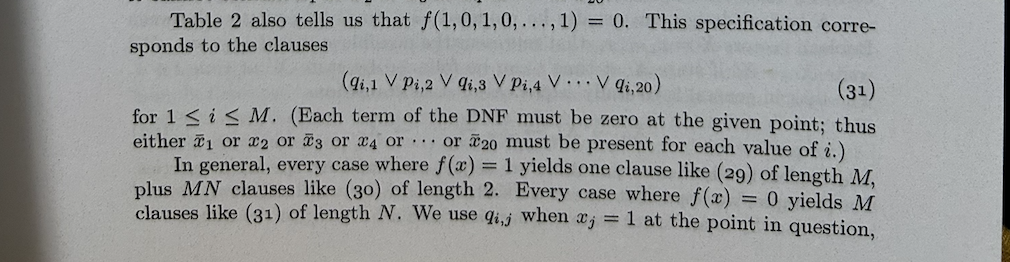
\includegraphics[width=130mm]{images/2-4.png}
\end{figure}
\begin{figure}[htbp]
  \centering
  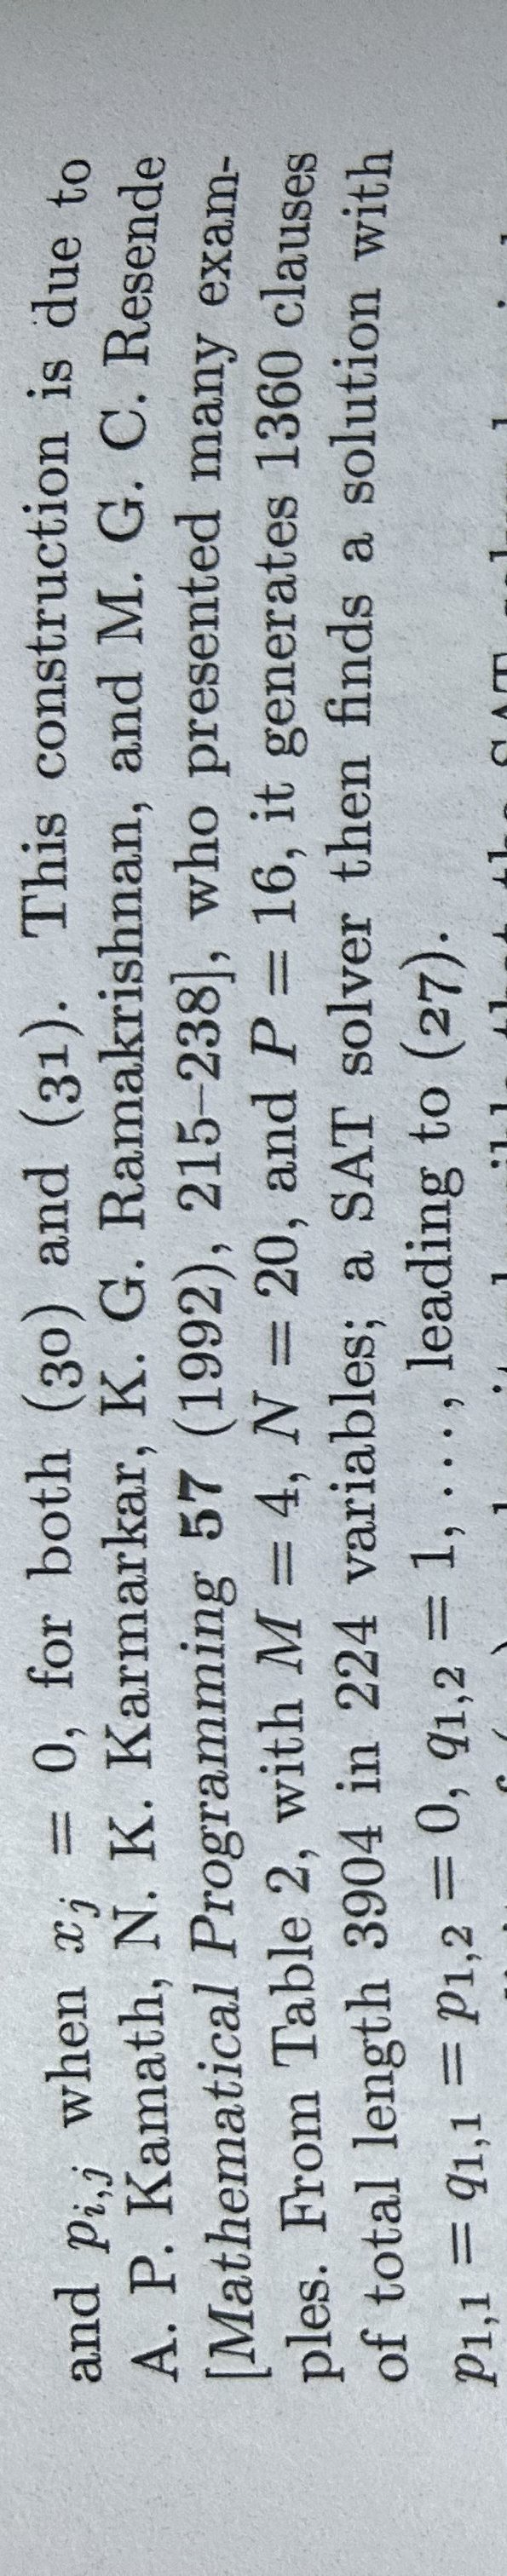
\includegraphics[width=26mm,angle=270]{images/3-1.jpg}
\end{figure}

表2はまた,$f(1,0,1,0,...,1)=0$であることも示している.この指定は対応する,節
  \begin{equation}
(q_{i,1} \lor p_{i,2} \lor q_{i,3} \lor p_{i,4} \lor ・・・ \lor q_{i,20})
\end{equation}  
に.$1 \le i \le M$に対して.
(DNFの各項は与えられた点で0でなければならない;それゆえ$\bar{x}_{1}$ or $x_{2}$ or $\bar{x}_{3}$ or $x_{4}$ or ・・・ or $\bar{x}_{20}$のいずれかが存在しなければならない,$i$の各値に対して.

一般に,$f(x) = 1$となる全ての場合で生じる,(29)のような長さ$M$の節が1つ,加えて(30)のような長さ2の節が$MN$.
$f(x) = 0$となる全ての場合で生じる,(31)のような長さ$N$の節が$M$.我々は$x_{j}=1$の時$q_{i,j}$を用いる,この問題の中でその点において,かつ$x_{j}=0$の時$p_{i,j}$を,(30)及び(31)の両方に.この構成はA. P. Kamath, N. K. Karmarkar, K. G. Ramakrishnan, and M. G. C. Resende (Mathematical Programming 57 (1992), 215-238) によるものである,(彼らは)多くの例を示している.表2より、$M = 4$, $N = 20$, $P = 16$で,それは1360の節を生み出す,合計の長さ3904で,224の変数を持つ;SATソルバーはその時解を求める,$p_{1,1}=q_{1,1}=p_{1,2}=1,...,$(27)を導く.

\begin{figure}[htbp]
  \centering
  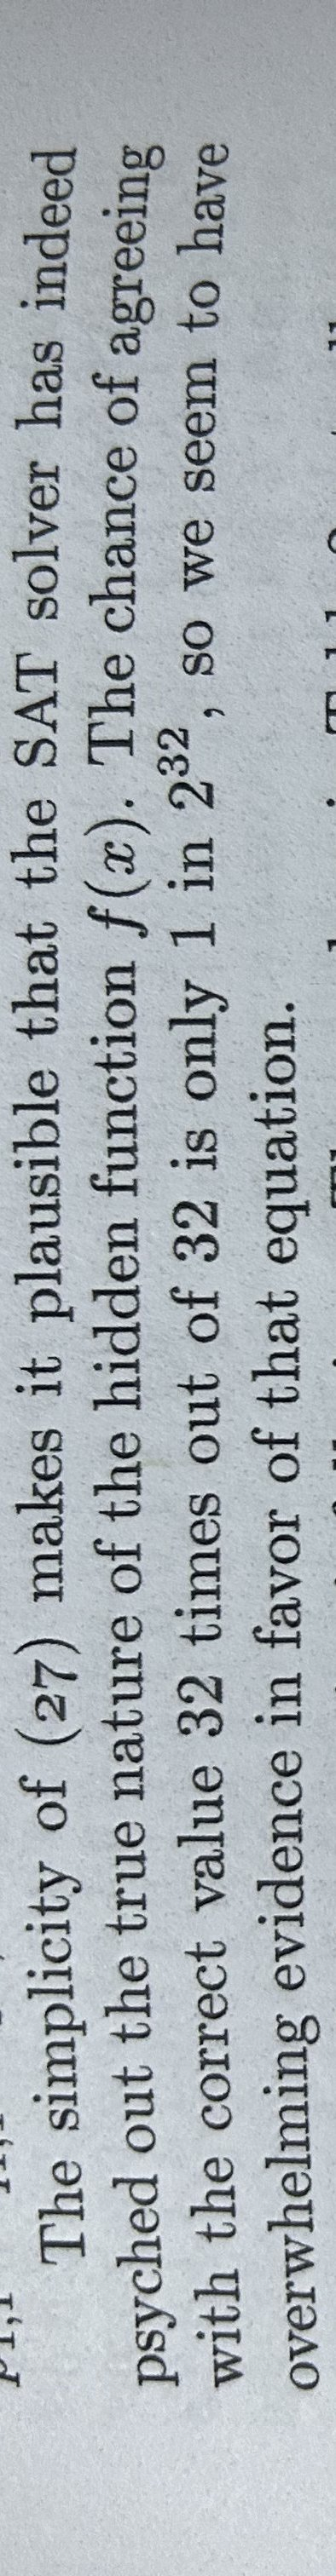
\includegraphics[width=17mm,angle=270]{images/3-2.jpg}
\end{figure}

(27)の単純性はそれを有力にする,SATソルバーが確かに隠れた関数$f(x)$の本質を見抜いたことを.32回中32回正しい値に一致する確率は$2^32$分の1なので,我々は圧倒的な証拠を持っていると言えるだろう,この等式を支持する.

\begin{figure}[htbp]
  \centering
  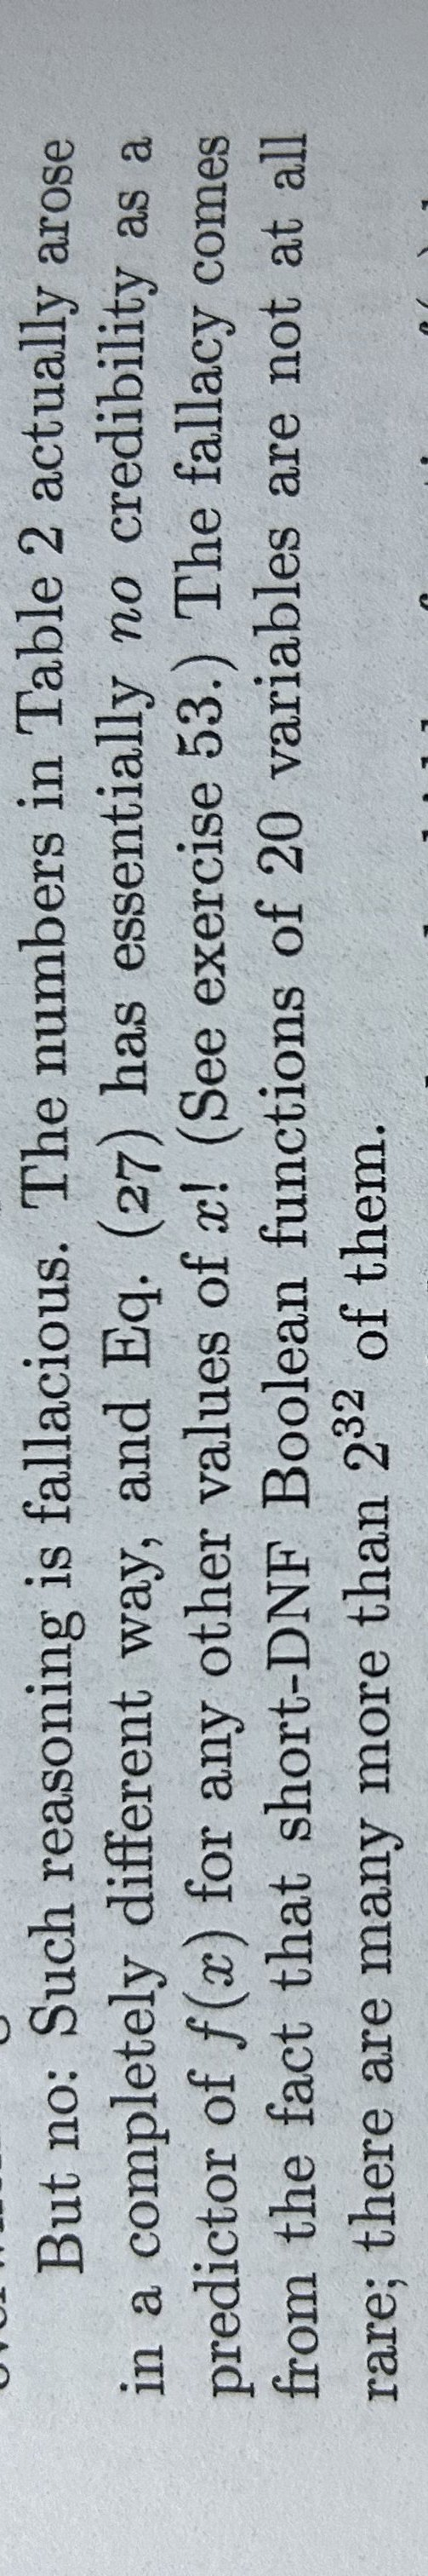
\includegraphics[width=22mm,angle=270]{images/3-3.jpg}
\end{figure}

 しかしそうではない:そのような推論は誤りである.表2の値は,実際にはまったく異なる方法と式により生じたものであり, (27)は,$f(x)$の予測因子として本質的に何の信頼もない,他のどのような$x$の値に対しても.(練習問題53を参照)この誤りは,20変数のshort-DNFブール関数が全く珍しいものではなく;$2^32$個より多く存在するという事実に起因する.
 \begin{figure}[htbp]
  \centering
  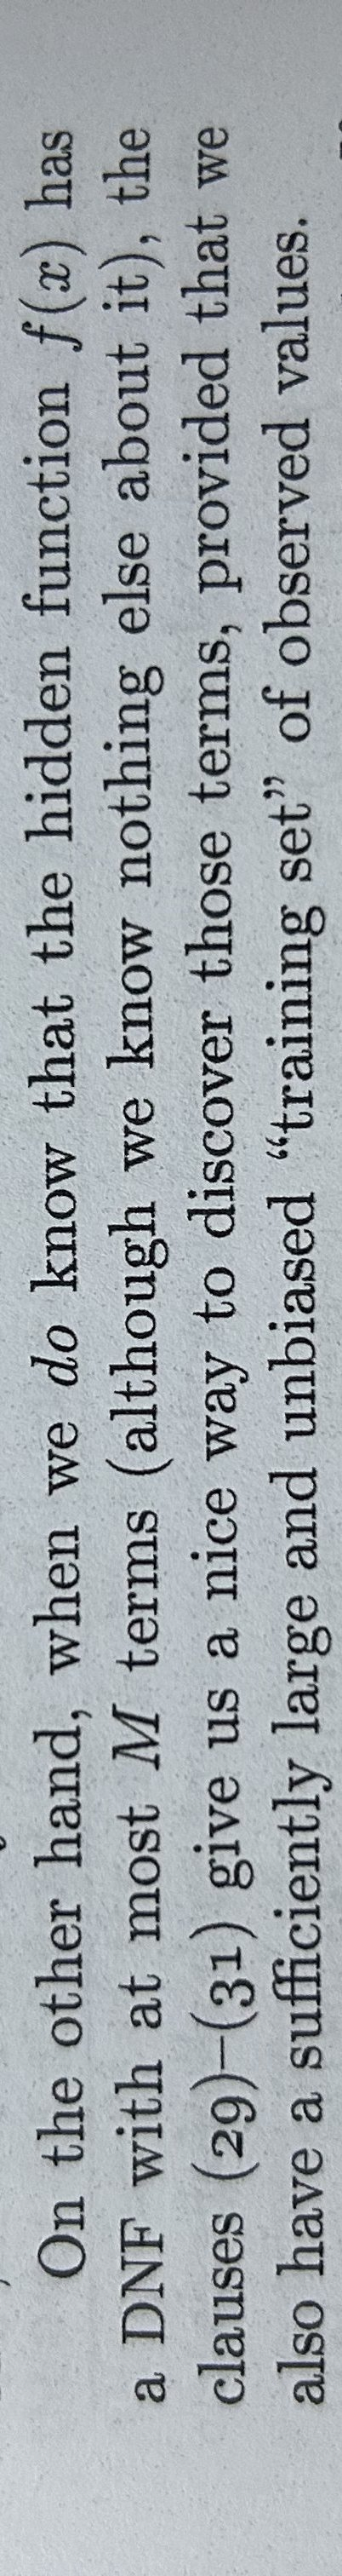
\includegraphics[width=18mm,angle=270]{images/3-4.jpg}
\end{figure}
一方で,隠れた関数$f(x)$が最大M個の項を持つDNFを持つことが分かっている場合(しかしそれ以外には何も分かっていない),節(29)-(31)は,我々にそれらの項を発見する良い方法を与えてくれる,十分に大きく偏りのない,値を観測する"訓練セット"を持っていれば.

 \begin{figure}[htbp]
  \centering
  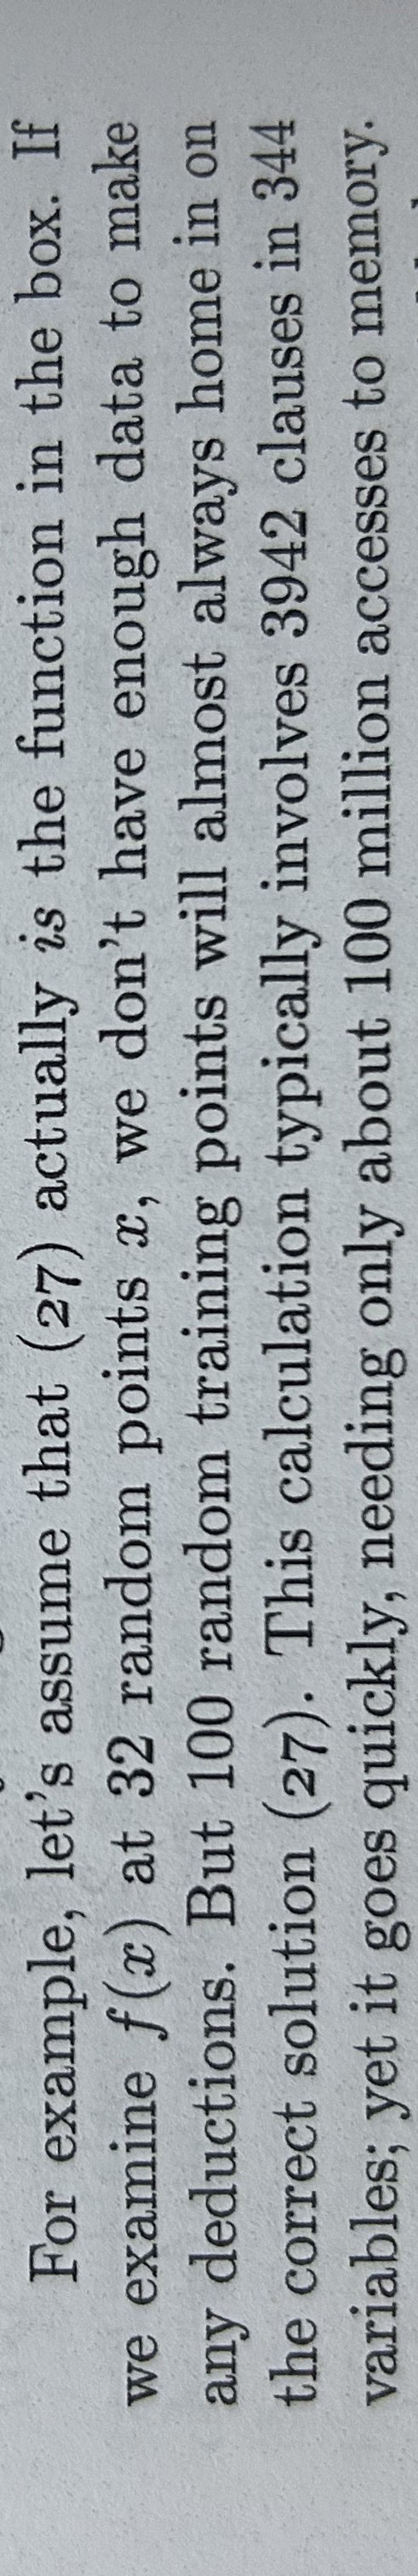
\includegraphics[width=22mm,angle=270]{images/3-5.jpg}
\end{figure}

例えば,(27)が実際に箱の中の関数であると仮定しよう.もし我々が32のランダムな点$x$で$f(x)$を調べても,我々は十分なデータを持っていない,どんな推論を行うにも.しかし100のランダムな学習点はほとんどいつも正しい解(27)にたどり着くだろう.この計算には通常344の変数と,3942の節が関わっている;しかしそれは早く,約1億回のメモリへのアクセスのみを必要とする.

%%%%%%%%%%%%%%%%%%%%%%%%%
\newpage

 \begin{figure}[htbp]
  \centering
  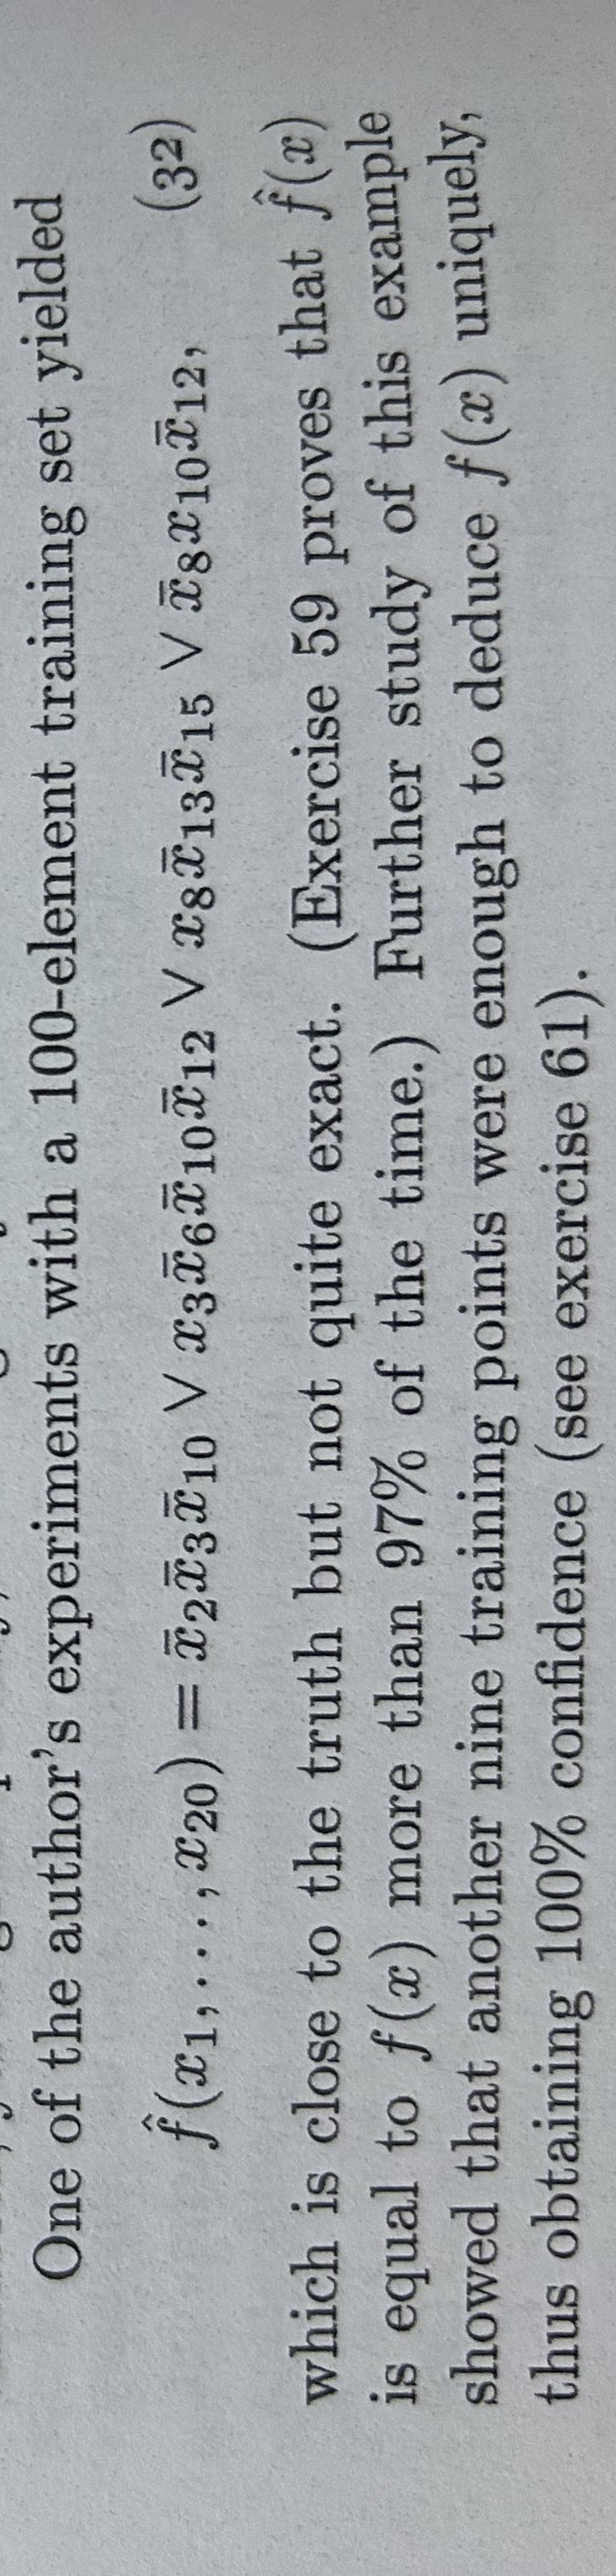
\includegraphics[width=32mm,angle=270]{images/3-6.jpg}
  \end{figure}
  100要素のトレーニングセットを用いた筆者の実験の1つは生み出した
  
  \begin{equation}
\hat{f}(x_{1},...,x_{20}) = \bar{x}_{2}\bar{x}_{3}\bar{x}_{10} \lor x_{3}\bar{x}_{6}\bar{x}_{10}\bar{x}_{12} \lor x_{8}\bar{x}_{13}\bar{x}_{15} \lor \bar{x}_{8}x_{10}\bar{x}_{12}, 
\end{equation}  
  
これは真実に近いが完全には正確でない.(練習問題59は$\hat{f}(x)$が97\%以上の$f(x)$と等しいことを示す.)この例題に対するさらなる研究は示した,他の9個の訓練点は$f(x)$を一意に推論するのに十分であり,従って100%の信頼性が得られた(練習問題61参照).



(本文のアルゴリズムを実際に行うプログラム:learning.py)

実行例:python learning.py input\_table2\_eq1.txt input\_table2\_eq0.txt 4
%%%%%%%%%%%%%%%%%%%%%%%%%
\newpage


\section*{Exercise 53}
\subsection*{問題}
 \begin{figure}[htbp]
  \centering
  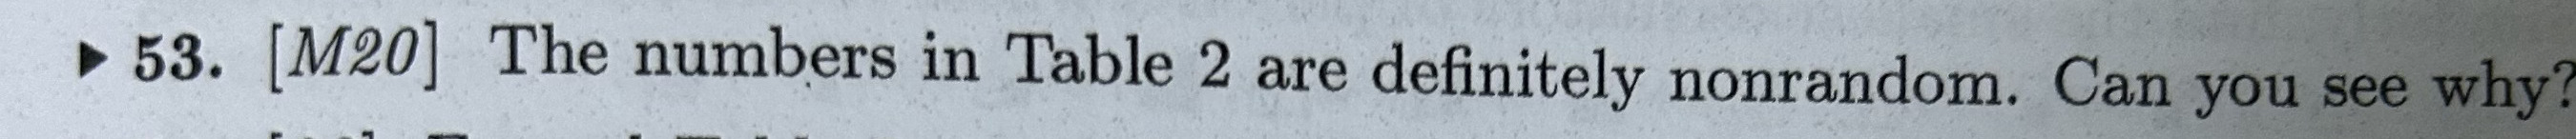
\includegraphics[width=142mm,angle=0]{images/51.jpg}
  \end{figure}
 表2の数字は明確に非ランダムである.あなたは何故か分かるだろうか.
 \subsection*{knuth先生の解答}
  \begin{figure}[htbp]
  \centering
  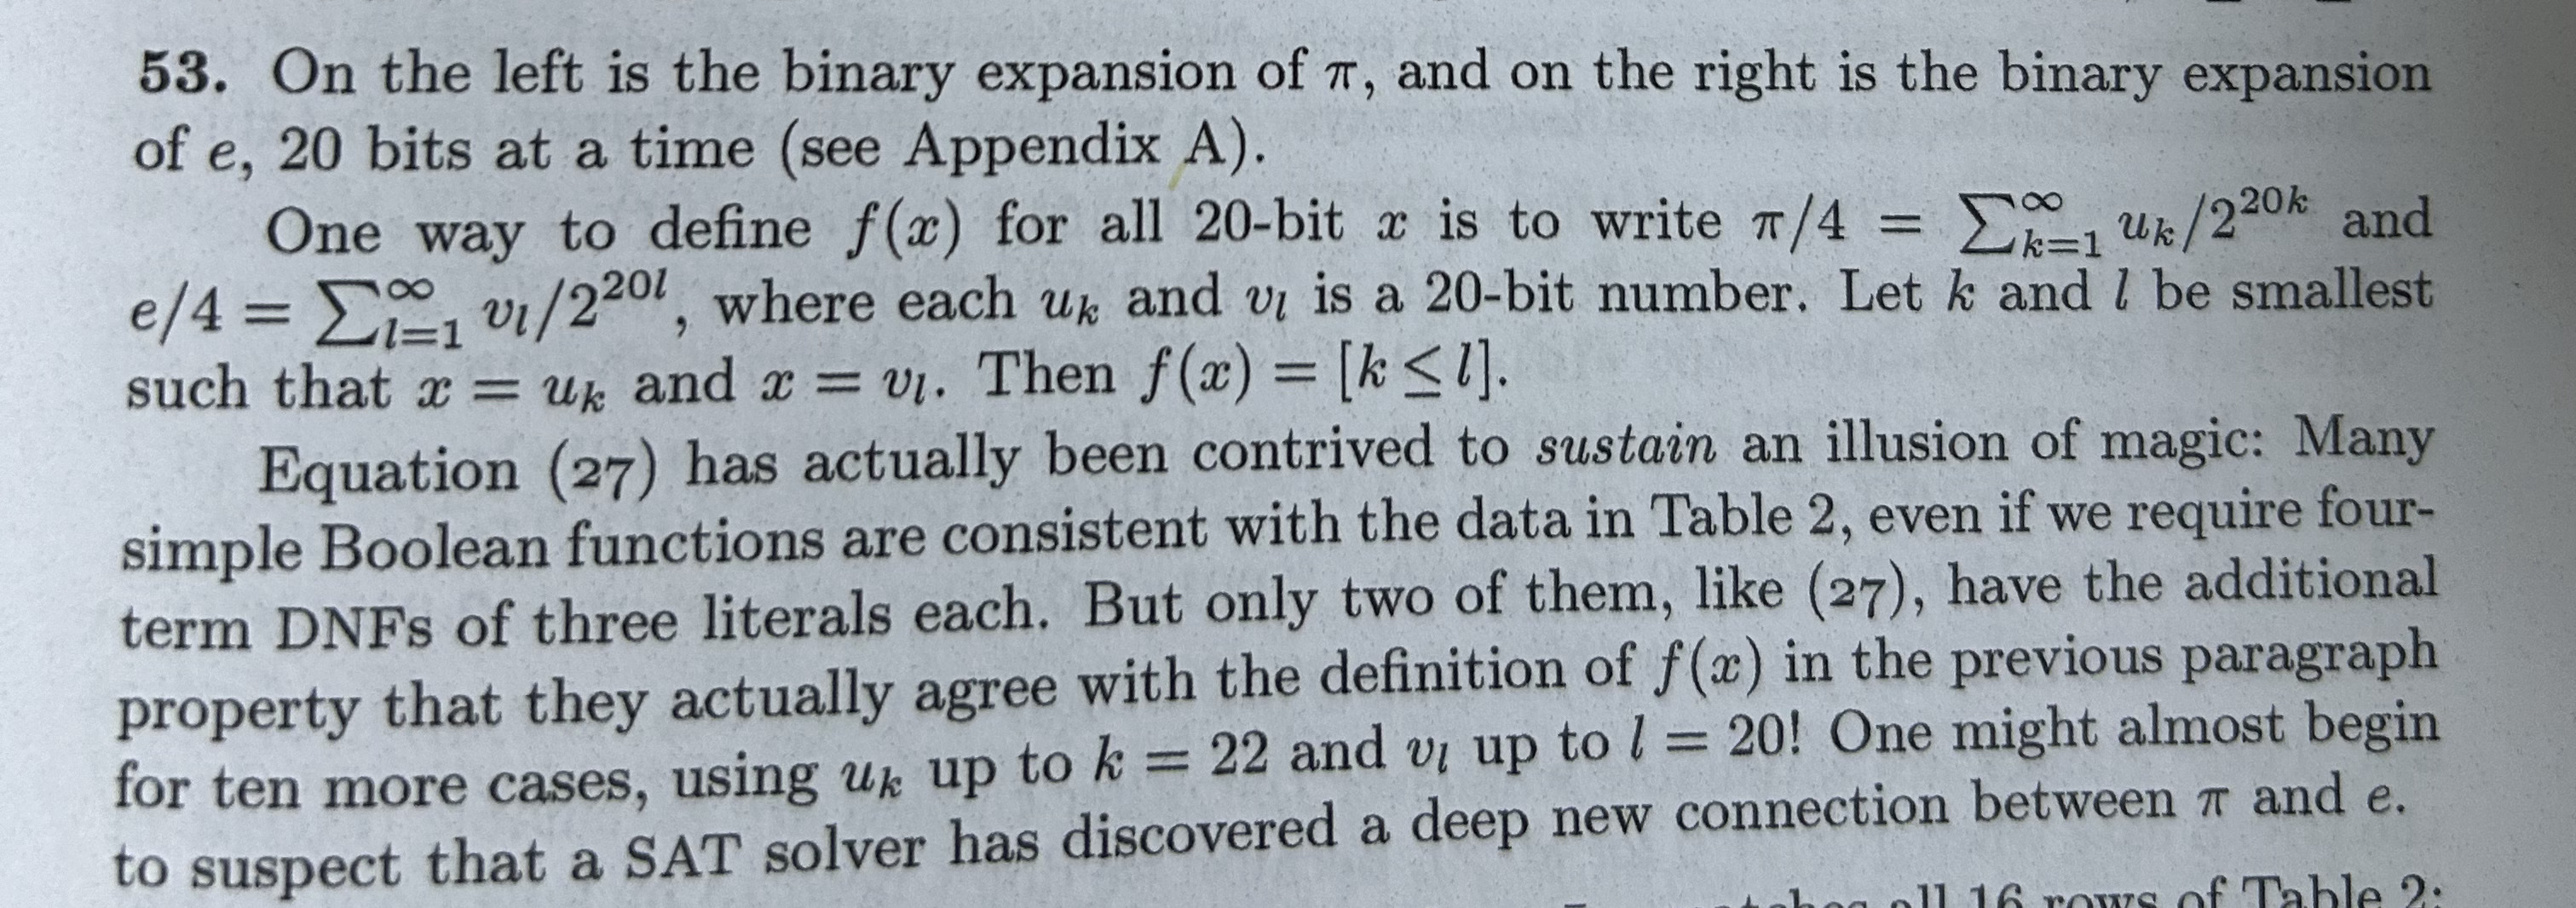
\includegraphics[width=142mm,angle=0]{images/53_a.jpg}
  \end{figure}
  
  
  
 左側は$π$の2進展開,右側は$e$の2進展開,一度に20ビットずつ.(付録A参照).
 
すべての20ビットの$x$に対して$f(x)$を定義する1つの方法は,$π/4 = \sum_{k=1}^\infty u_{k}/2^{20k}$ と $e/4 = \sum_{l=1}^\infty v_{l}/2^{20l}$ を記述することである,
ここで各$u_{k}$と$v_{l}$は20ビットの数である.$x=u_{k}$かつ$x=v_{l}$となるような$k$と$l$を最小にしてみよう.
その時,$f(x) = [k \leq l]$

式(27)は、実際には魔法のような錯覚を持続させるために考案されたものである:多くの単純なブール関数は表2のデータと一致する,3リテラルずつの4項のDNFを必要とするとしても.しかし,そのうち2つだけが,(27)のように,追加的な性質を持っている,それらが$k=22$までの$u_{k}$と$l=20$までの$v_{l}$を使った10以上のケースについて,前の段落の$f(x)$の定義と実際に一致するという.誰かは疑い始めてしまうかもしれない,SATソルバーが$π$と$e$の間に新しく深い関係を発見したのではないかと.

   \begin{figure}[htbp]
  \centering
  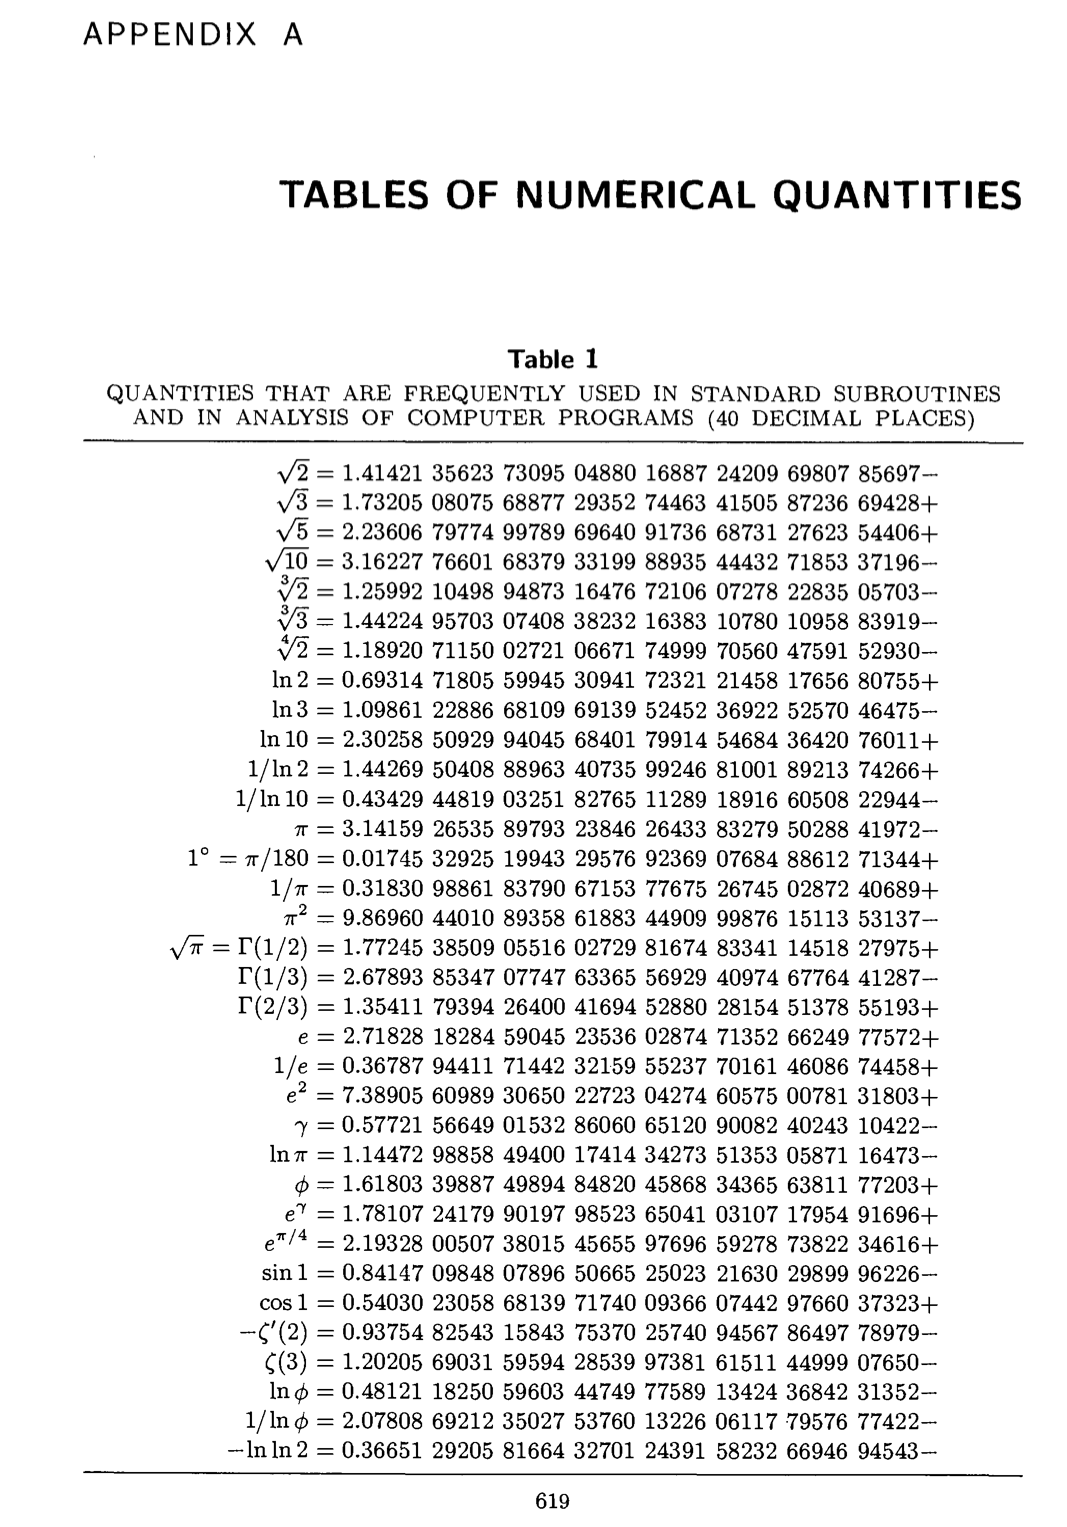
\includegraphics[width=142mm,angle=0]{images/appen.png}
  \end{figure}

\newpage
 \subsection*{自身の解答}
 \begin{enumerate}
 
\item  $π/4 = \sum_{k=1}^\infty u_{k}/2^{20k}$ は,$π/4$を2進数に変換し,上の桁から20ビットずつ切り出すことを表している.(e/4の方も同様)
 
\begin{itemize}
\item 実際に計算するプログラム:ex53\_1.py
\item 実行例:python ex53\_1.py -pi 320
\end{itemize}

\item $x=u_{k}$かつ$x=v_{l}$となるような$k$と$l$を探索する
\begin{itemize}
\item プログラム:ex53\_2.py
\item 実行例:python ex53\_2.py 32000
\end{itemize}

\item  $k=17..22$の$u_{k}$と$l=17..20$の$v_{l}$において表2の$f(x)$の定義と一致する(=すなわち,$u_{k}$の20ビットを$x$とすると$f(x)$=1となり,$v_{l}$の20ビットを$x$とすると$f(x)$=0となる)

\begin{itemize}
\item プログラム:ex53\_3.py
\item 実行例:python ex53\_3.py 11101111100101010001
\end{itemize}




 \end{enumerate}
 
  \begin{table}[h]
 \caption{$u_{k}(k=17..23)$}
 {\scriptsize
 \hspace{4cm}
 \begin{tabular}{l|r|r}
 $k$ & $u_{k}$ & $f(x)$  \\ \hline
 17 & 11101111100101010001 & 1 \\
 18 &10011011001111001101 & 1\\
19 &00111010010000110001 &1 \\
20 &10110011000000101011&1\\
21 &00001010011011011111&1\\
22 &00100101111100010100&1\\
23 &00110111010011111110&0\\
\end{tabular}
 }
 \end{table}
 
  \begin{table}[h]
 \caption{$v_{l}(l=17..21)$}
 {\scriptsize
 \hspace{4cm}
 \begin{tabular}{l|r|r}

 $l$ & $v_{l}$ & $f(x)$  \\ \hline
17 &01111101001011111110 & 0\\
18 &00110110001101100011&0\\
19 &00001100011101011101&0\\
20 &10001111011010000001&0\\
21 &10110010000000101010&1 \\
\end{tabular}
 }
 \end{table}


  %%%%%%%%%%%%%%%%%%%%%%%%%
  
\newpage
\section*{Exercise 59}
\subsection*{問題}
 \begin{figure}[htbp]
  \centering
  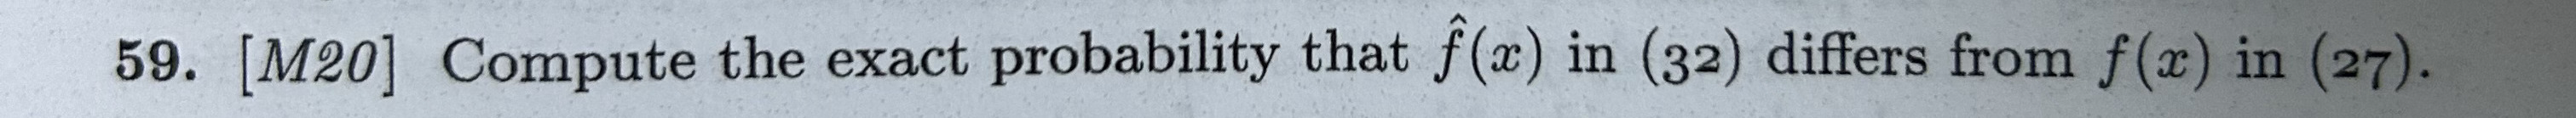
\includegraphics[width=142mm,angle=0]{images/59.jpg}
  \end{figure}
  (32)の$\hat{f(x)}$が(27)の$f(x)$と異なる正確な確率を計算せよ.
  
  (任意の入力$x$に対し,$f(x) \neq \hat{f(x)}$となる確率)

 \subsection*{knuth先生の解答}
 \begin{figure}[htbp]
  \centering
  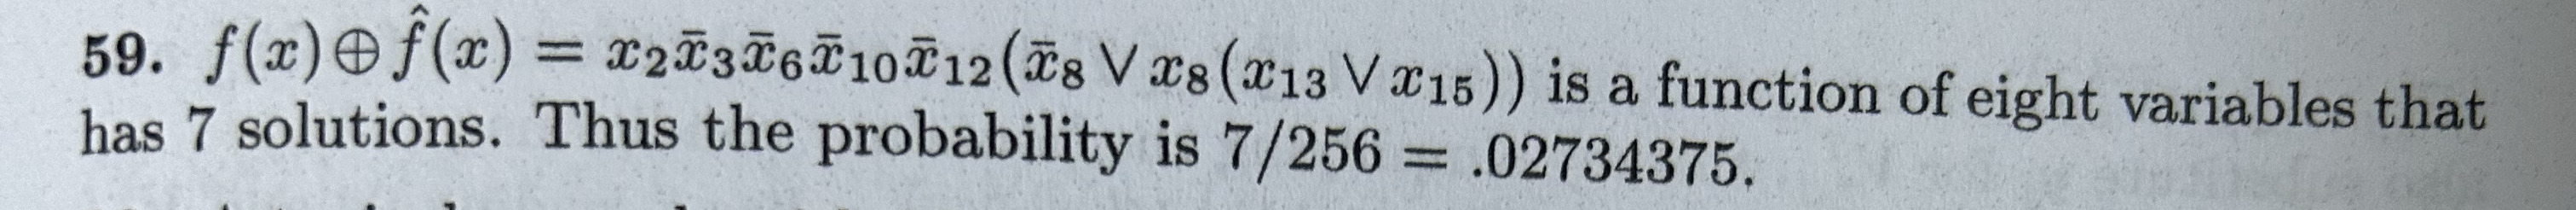
\includegraphics[width=142mm,angle=0]{images/59a.jpg}
  \end{figure}
  
  $f(x) \oplus \hat{f(x)} = x_{2}\bar{x}_{3}\bar{x}_{6}\bar{x}_{10}\bar{x}_{12}(\bar{x}_{8} \lor x_{8} (x_{13} \lor x_{15}))$
  は8変数の関数で,7つの解を持つ.したがって確率は7/256 = .02734375である.

 \subsection*{自身の解答}
 $f(x) \neq \hat{f(x)}$となるような入力$x$の総数を計算する.
 $f(x) \oplus \hat{f(x)}=1$となれば良いので,まず$f(x) \oplus \hat{f(x)}$を考える.
  
 \begin{gather*}
f(x) = \bar{x}_{2}\bar{x}_{3}\bar{x}_{10}\lor\bar{x}_{6}\bar{x}_{10}\bar{x}_{12}\lor x_{8}\bar{x}_{13}\bar{x}_{15}\lor \bar{x}_{8}x_{10}\bar{x}_{12} \\
\hat{f}(x) = \bar{x}_{2}\bar{x}_{3}\bar{x}_{10} \lor x_{3}\bar{x}_{6}\bar{x}_{10}\bar{x}_{12} \lor x_{8}\bar{x}_{13}\bar{x}_{15} \lor \bar{x}_{8}x_{10}\bar{x}_{12}
\end{gather*}  
ここで,
 \begin{gather*}
A = \bar{x}_{2}\bar{x}_{3}\bar{x}_{10}\lor x_{8}\bar{x}_{13}\bar{x}_{15}\lor \bar{x}_{8}x_{10}\bar{x}_{12} \\
B  = \bar{x}_{6}\bar{x}_{10}\bar{x}_{12} 
\end{gather*}  
と置くと,
\begin{gather*}
f(x) = A \lor B \\
\hat{f}(x) = A \lor x_{3}B 
\end{gather*}  
と表せる.
\begin{gather*}
f(x) \oplus \hat{f(x)} = f(x)\overline{\hat{f(x)}} \lor \overline{f(x)}\hat{f(x)} 
\end{gather*}  
より,まず $f(x)\overline{\hat{f(x)}}$について考える.
\begin{align*}
f(x)\overline{\hat{f(x)}}  & = (A \lor B)・\overline{(A \lor x_{3}B)} \\
& = (A \lor B)・(\bar{A} ・(\bar{x}_{3} \lor \bar{B})) \\
& = (A \lor B)・(\bar{x}_{3}\bar{A} \lor \bar{A}\bar{B}) \\
& = \bar{x}_{3}A\bar{A} \lor A\bar{A}\bar{B} \lor \bar{x}_{3}\bar{A}\bar{B} \lor \bar{A}\bar{B}B \\
& = \bar{x}_{3}\bar{A}B \tag{i}
\end{align*}  
次に,$\overline{f(x)}\hat{f(x)}$について考える.
\begin{align*}
\overline{f(x)}\hat{f(x)}  & = \overline{(A \lor B)}・(A \lor x_{3}B) \\
& = \bar{A}\bar{B}・(A \lor x_{3}B) \\
& = \bar{A}\bar{B}A \lor  \bar{A}\bar{B}x_{3}B \\
& = 0 \tag{ii}
\end{align*}  
(i),(ii)より,
\begin{gather*}
f(x) \oplus \hat{f(x)} =  \bar{x}_{3}\bar{A}B 
\end{gather*}  
\begin{align*}
 \bar{x}_{3}\bar{A}B &= \bar{x}_{3}・(\overline{\bar{x}_{2}\bar{x}_{3}\bar{x}_{10}\lor x_{8}\bar{x}_{13}\bar{x}_{15}\lor \bar{x}_{8}x_{10}\bar{x}_{12}})・(\bar{x}_{6}\bar{x}_{10}\bar{x}_{12}) \\
 & = \bar{x}_{3}・(\overline{\bar{x}_{2}\bar{x}_{3}\bar{x}_{10}}・ \overline{x_{8}\bar{x}_{13}\bar{x}_{15}}・ \overline{\bar{x}_{8}x_{10}\bar{x}_{12}})・(\bar{x}_{6}\bar{x}_{10}\bar{x}_{12}) \\
 & = \bar{x}_{3}\bar{x}_{6}\bar{x}_{10}\bar{x}_{12}・(x_{2} \lor x_{3} \lor x_{10})・(\bar{x}_{8} \lor x_{13} \lor x_{15})・(x_{8} \lor \bar{x}_{10} \lor x_{12}) \\
 & = (\bar{x}_{3}\bar{x}_{6}\bar{x}_{10}\bar{x}_{12} \lor \bar{x}_{3}\bar{x}_{6}\bar{x}_{10}\bar{x}_{12}x_{2}x_{3} \lor \bar{x}_{3}\bar{x}_{6}\bar{x}_{10}\bar{x}_{12}x_{2}x_{10})・(\bar{x}_{8} \lor x_{13} \lor x_{15})・(x_{8} \lor \bar{x}_{10} \lor x_{12}) \\
& = x_{2} \bar{x}_{3}\bar{x}_{6}\bar{x}_{10}\bar{x}_{12}・(\bar{x}_{8} \lor x_{13} \lor x_{15})・(x_{8} \lor \bar{x}_{10} \lor x_{12}) \\
& = (x_{2} \bar{x}_{3}\bar{x}_{6}\bar{x}_{10}\bar{x}_{12}\bar{x}_{8} \lor x_{2} \bar{x}_{3}\bar{x}_{6}\bar{x}_{10}\bar{x}_{12}x_{13} \lor x_{2} \bar{x}_{3}\bar{x}_{6}\bar{x}_{10}\bar{x}_{12}x_{15})・(x_{8} \lor \bar{x}_{10} \lor x_{12}) \\
& = x_{2}\bar{x}_{3}\bar{x}_{6}\bar{x}_{10}\bar{x}_{12}\bar{x}_{8}x_{8} \lor x_{2} \bar{x}_{3}\bar{x}_{6}\bar{x}_{10}\bar{x}_{12}x_{13}x_{8} \lor x_{2} \bar{x}_{3}\bar{x}_{6}\bar{x}_{10}\bar{x}_{12}x_{15}x_{8}  \\
 & \lor x_{2} \bar{x}_{3}\bar{x}_{6}\bar{x}_{10}\bar{x}_{12}\bar{x}_{8}\bar{x}_{10} \lor x_{2} \bar{x}_{3}\bar{x}_{6}\bar{x}_{10}\bar{x}_{12}x_{13}\bar{x}_{10} \lor x_{2} \bar{x}_{3}\bar{x}_{6}\bar{x}_{10}\bar{x}_{12}x_{15}\bar{x}_{10} \\
 &  \lor x_{2} \bar{x}_{3}\bar{x}_{6}\bar{x}_{10}\bar{x}_{12}\bar{x}_{8}x_{12} \lor x_{2} \bar{x}_{3}\bar{x}_{6}\bar{x}_{10}\bar{x}_{12}x_{13}x_{12} \lor x_{2} \bar{x}_{3}\bar{x}_{6}\bar{x}_{10}\bar{x}_{12}x_{15}x_{12} \\
 & =   x_{2} \bar{x}_{3}\bar{x}_{6}\bar{x}_{10}\bar{x}_{12}x_{13}x_{8} \lor x_{2} \bar{x}_{3}\bar{x}_{6}\bar{x}_{10}\bar{x}_{12}x_{15}x_{8}  \lor x_{2} \bar{x}_{3}\bar{x}_{6}\bar{x}_{10}\bar{x}_{12}\bar{x}_{8} \\
 &  \lor x_{2} \bar{x}_{3}\bar{x}_{6}\bar{x}_{10}\bar{x}_{12}x_{13} \lor x_{2} \bar{x}_{3}\bar{x}_{6}\bar{x}_{10}\bar{x}_{12}x_{15} \\
 & =   x_{2}\bar{x}_{3}\bar{x}_{6}\bar{x}_{10}\bar{x}_{12}(x_{13}x_{8} \lor x_{15}x_{8}  \lor \bar{x}_{8} \lor x_{13} \lor x_{15}) \\
 & =   x_{2}\bar{x}_{3}\bar{x}_{6}\bar{x}_{10}\bar{x}_{12}(\bar{x}_{8} \lor x_{13} \lor x_{15}) \\
 \end{align*}  
 したがって,
 \begin{gather*}
f(x) \oplus \hat{f(x)} =  x_{2}\bar{x}_{3}\bar{x}_{6}\bar{x}_{10}\bar{x}_{12}(\bar{x}_{8} \lor x_{13} \lor x_{15})
\end{gather*}  
この論理式には変数が8つ存在し,$f(x) \oplus \hat{f(x)} = 1$となる変数の値割り当ては7通り($x_{2}=1,x_{3}=0,x_{6}=0,x_{10}=0,x_{12}=0$かつ,$\bar{x}_{8},x_{13},x_{15}$のうち1つ以上が真となれば良いので$2^3-1=7$通り).
それに対し,変数の値割り当ての総数は$2^8=256$.

よって,求める確率は$7/256 \simeq 0.02734375$.
 
  
%%%%%%%%%%%%%%%%%%%%%%%%%
\section*{Exercise 61}
 \begin{figure}[htbp]
  \centering
  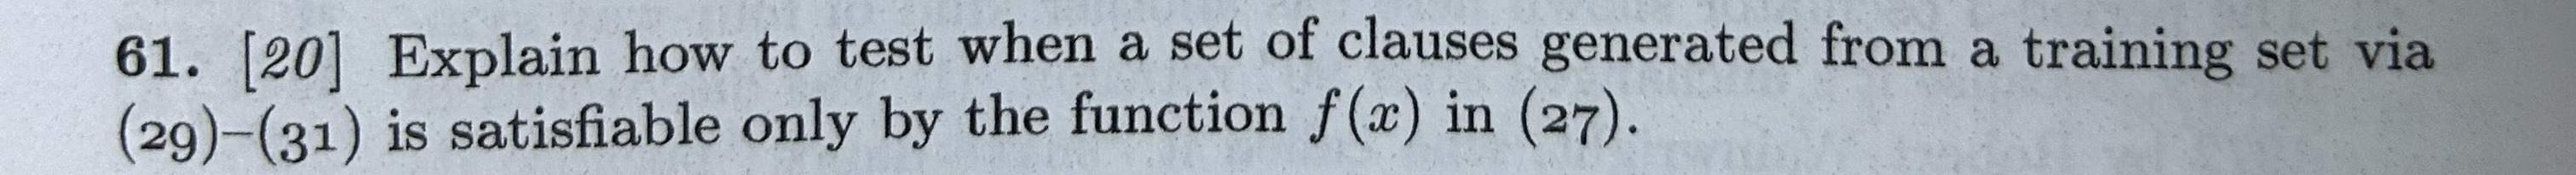
\includegraphics[width=142mm,angle=0]{images/61.jpg}
  \end{figure}

 \begin{figure}[htbp]
  \centering
  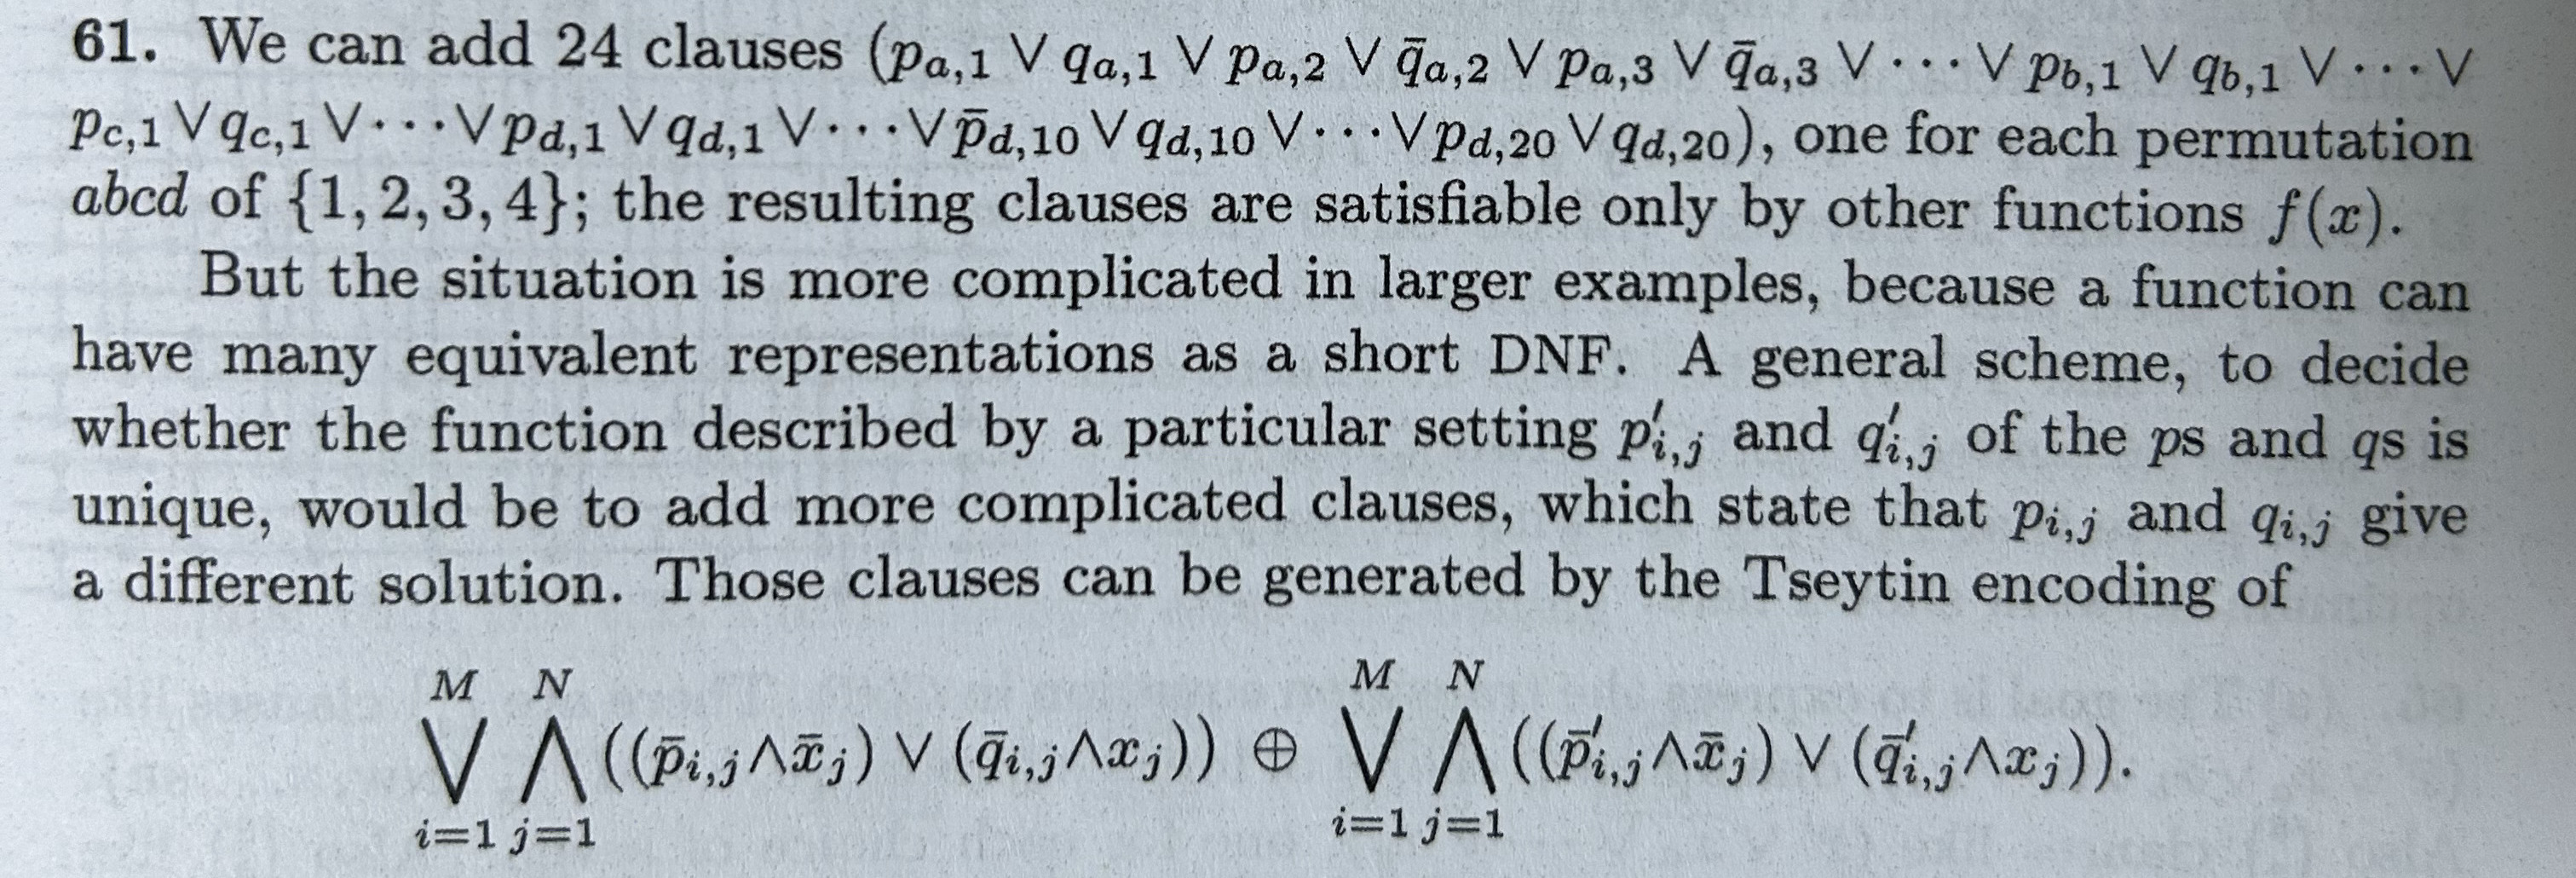
\includegraphics[width=142mm,angle=0]{images/61a.jpg}
  \end{figure}

  

\end{document}
